\section{Trapping Configurations}
Now that we have a better understanding of the types of ions used in trapped ion quantum computing, as well as some of the advantages and disadvantages they each have, we can turn our attention to the trapping configurations. 

When considering the possible geometries that an ion trap can have, we're essentially given two choices: one-dimensional (1D), also known as linear arrays; or two-dimensional (2D), sometimes called planar arrays, which is the basis for the 2D Coulomb crystals we're building up to. 

\subsection{Linear Arrays}
It may come as no surprise that the first quantum computers to be described using trapped ions made use of linear traps. Despite the simplistic geometry, all the necessary features of a quantum computer can be realized with linear ion traps. It's even possible to implement quantum gates between any set of ions in this scheme, not necessarily neighboring ions, for gates involving pairs, triplets, or any arbitrary number of ions. However, in practice, increasing the number of effective qubits is not an arbitrary task. Decoherence due to the environment interacting with the quantum system remains a significant challenge \cite{Cirac}.

Nevertheless, advances have been made that show how quantum computers based on linear arrays could provide solutions to difficult problems in materials design and molecular modeling through quantum simulation. In one example from 2017, Zhang \textit{et al.} successfully performed a quantum simulation of a dynamical phase transition (DPT) using up to 53 qubits in a linear ion trap. In this system, the qubits are coupled at long-range through their collective quantized motion due to Coulomb interactions. Each individual qubit is measured by a global long-range Ising interaction which has an efficiency of almost 99\%. This high efficiency makes it possible to measure many-body correlations between qubits in one shot, thereby allowing the DPT to be probed directly \cite{Zhang}.

The method employed by Zhang \textit{et al.} for confinement of long ion chains relied on a three-layer linear Paul trap with \ion{171}{Yb}{+} ions. Across the chain, ion spacing is anisotropic, ranging from \SI{1.5}{\micro\meter} at the center to \SI{3.5}{\micro\meter} towards the ends. As one might expect, the average lifetime of the chain scales inversely with the number of ions. At the maximum, 53 ions, an average lifetime of about 5 minutes was observed (which was sufficient for this experiment). The greatest factor in limiting the effective liftetime of the ion chain was Langevin collisions with residual background gas. When looking to scale up a system of this type, it will be crucial to implement cryogenic trap systems to reduce the pressure and collision energies \cite{Zhang}. 

More recently, a flexible scheme for maintaining efficient entanglement between ions in a long chain as the size scales up has been introduced by Leung and Brown. By utilizing both amplitude and frequency modulation, they show it's theoretically possible to apply high-fidelity pulse sequences to drive transverse motional modes, which can suppress gate errors (See Fig. \ref{fig:Linear Trap}). Those pulses in turn require greater power to operate, so there is a trade-off between higher tolerance against errors and power efficiency.

\begin{figure}[h]
    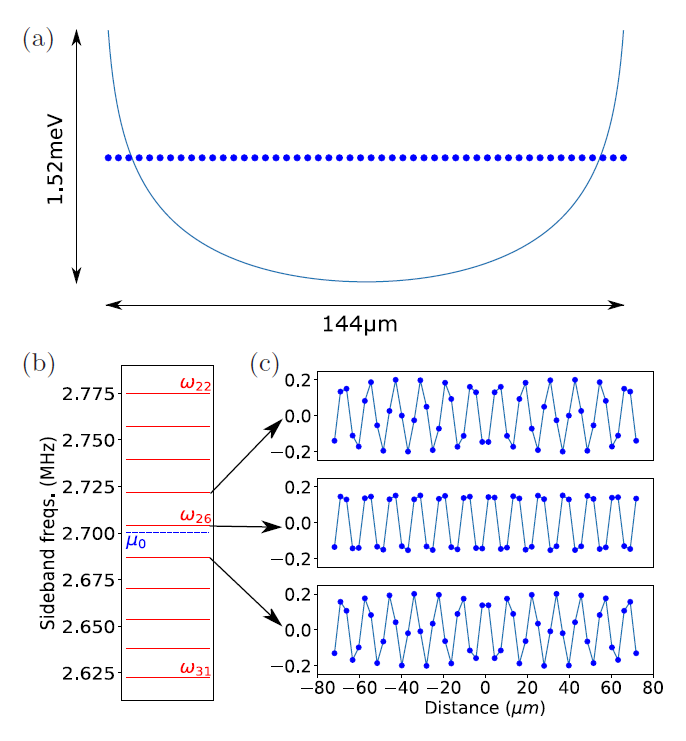
\includegraphics[width=\linewidth]{Leung - Linear Trap.png}
    \caption{(\textbf{a}) An idealized distribution of ions in a trap with $r=0.95$. The minimum trap depth required to trap all 50 ions is \SI{1.52}{\milli\electronvolt}. (\textbf{b}) The middle band of the transverse motional frequencies. The approximate driving frequency is represented by the dashed blue line where $\mu_0 = \omega_{26} - \SI{3.7}{\kilo\hertz}$. (\textbf{c}) The normalized 25th to 27th transverse motional modes. In the center is the 26th mode which exhibits a valuable unformity making it an excellent candidate for two-qubit entanglement. From \textit{Entangling an arbitrary pair of qubits in a long ion crystal} \cite{Leung}.}
    \label{fig:Linear Trap}
\end{figure}

While linear arrays remain a promising area of research, there are some shortcomings to this particular trap geometry. In general, as the size of the ion chain increases, there is weaker motional coupling between ions with ion-ion coupling strength falling off as $1/s^\alpha$ where $s$ is the distance between two ions. That then leads to limitations such as decreasing speed of qubit gates and a corresponding increase in noise-induced heating in the system (due to the gates taking longer) \cite{Bruzewicz}.

Those challenges could be overcome if the ion chain were to be broken into smaller pieces, or modules, which could perform operations at high-speed and efficacy within an individual module. That type of scheme would require some way of moving the quantum information between modules or even moving the ions themselves. This is possible given variable voltages in the ion trap electrodes that control the trapping potential. We can imagine breaking off subsets of ions from their modules and combining them in a new module to allow interaction. Then by returning them to their original positions, that quantum information has become more widely distributed. However, this process of splitting and joining many ion chains comes with it's own challenges and the ability to do it quickly and with high fidelity will be constrained by the size of the ion chain \cite{Bruzewicz}.

While distribution of quantum information is not impossible in a 1D linear array (and quantum computing is certainly possible), there are improvements that can be made in some areas by expanding to a 2-dimensional array.

\subsection{Planar Arrays}
Two-dimensional or planar arrays are built on the same concepts as the linear arrays we just discussed: Radio-frequency traps are utilized to hold atomic ions in an electric potential where they can be coupled and controlled by applying precise laser beams. However, working in two dimesions presents additional advantages along with a unique set of challenges. The move into two dimensions also brings us into the realm of 2D Coulomb crystals which will be the focus of the remainder of this paper.

When looking to scale up trapped-ion systems, 2D architectures have been proposed to mitigate the problems faced by larger linear arrays. In a linear chain, the ions are only weakly confined along the axial direction of the chain. Because of this, high heating rates can occur due to the axial motional modes making laser cooling a challenge. It also becomes a issue for laser-addressing the outer ions as the length of an ion chain grows. Just keeping a long one-dimensional chain in a linear form requires extremely anisotropic traps that ultimately limit how many ions can be controlled without introducing errors. Introducing a second spatial dimension can be shown to overcome these obstacles related to heating, quantum state manipulation, and more \cite{Wang,Kiesenhofer}.

In 2023, Kiesenhofer \textit{et al.} introduced a novel ion-trap apparatus that could achieve quantum control over planar ion crystals of up to 105 ions while 

I have reset the sensors to scan for frequencies outside the usual range. By emitting harmonic vibrations to shatter the lattices. We will monitor and adjust the frequency of the resonators. He has this ability of instantly interpreting and extrapolating any verbal communication he hears. It may be due to the envelope over the structure, causing hydrogen-carbon helix patterns throughout. I'm comparing the molecular integrity of that bubble against our phasers.

We're acquainted with the wormhole phenomenon, but this... Is a remarkable piece of bio-electronic engineering by which I see much of the EM spectrum ranging from heat and infrared through radio waves, et cetera, and forgive me if I've said and listened to this a thousand times. This planet's interior heat provides an abundance of geothermal energy. We need to neutralize the homing signal.

Communication is not possible. The shuttle has no power. Using the gravitational pull of a star to slingshot back in time? We are going to Starbase Montgomery for Engineering consultations prompted by minor read-out anomalies. Probes have recorded unusual levels of geological activity in all five planetary systems. Assemble a team. Look at records of the Drema quadrant. Would these scans detect artificial transmissions as well as natural signals?

Exceeding reaction chamber thermal limit. We have begun power-supply calibration. Force fields have been established on all turbo lifts and crawlways. Computer, run a level-two diagnostic on warp-drive systems. Antimatter containment positive. Warp drive within normal parameters. I read an ion trail characteristic of a freighter escape pod. The bomb had a molecular-decay detonator. Detecting some unusual fluctuations in subspace frequencies.

Resistance is futile.